\documentclass{standalone}
\usepackage{tikz}
\usetikzlibrary{patterns, positioning}

\begin{document}
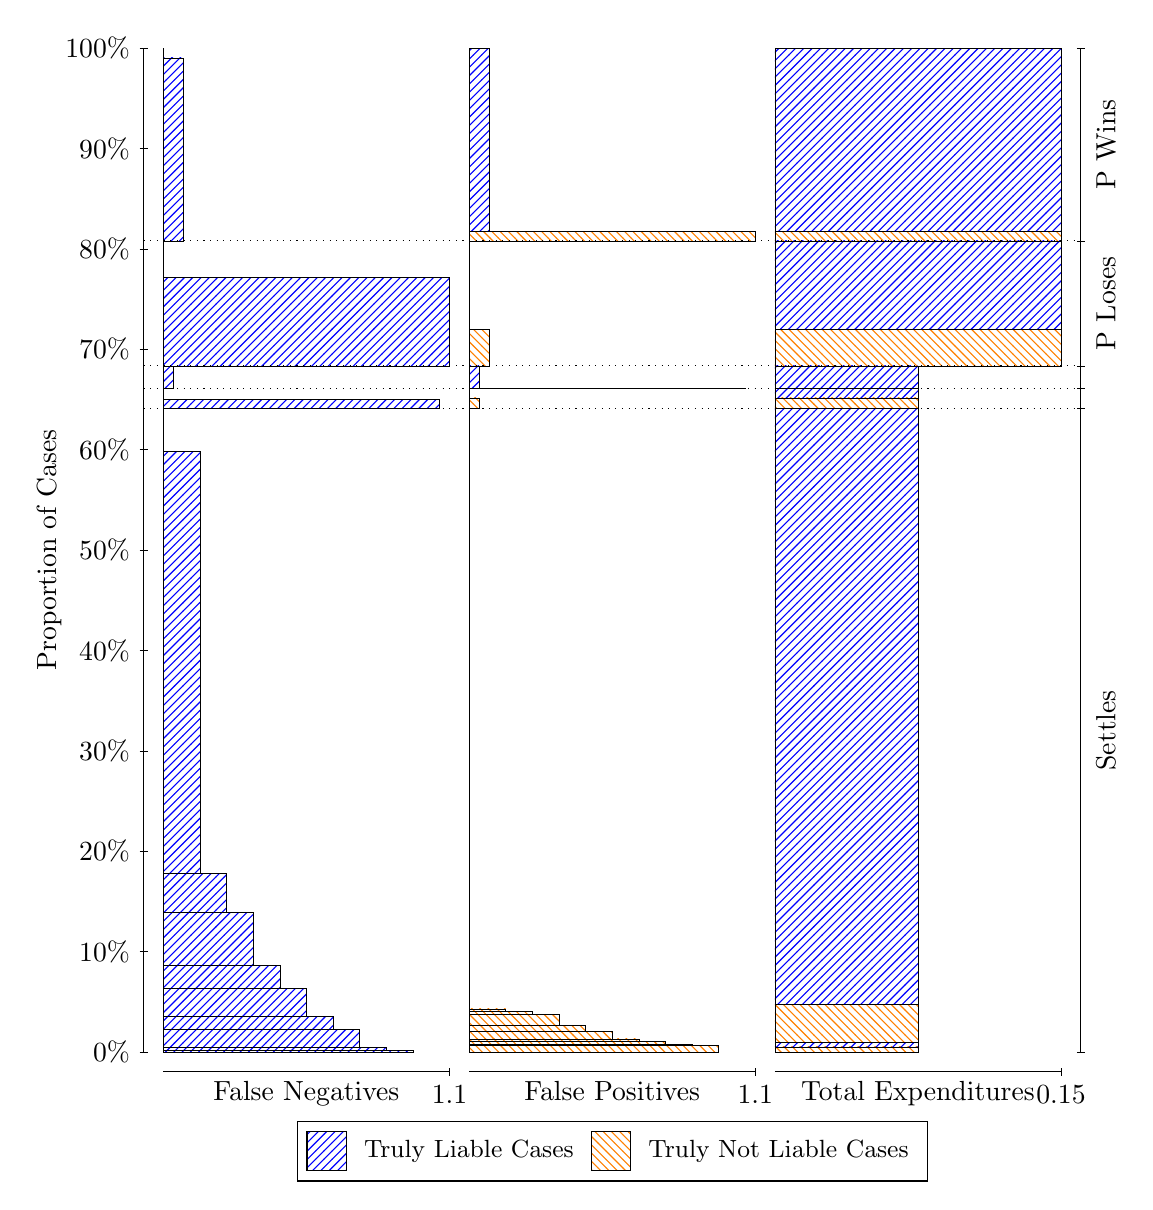
\begin{tikzpicture}
\draw[black, very thin] (1.5,1.75) -- (1.5,14.5);
\node[rotate=90, anchor=center] at (0.3, 8.125) {Proportion of Cases};
\draw[black, very thin] (1.45,1.75) -- (1.55,1.75);
\node[anchor=east] at (1.45, 1.75) {0\%};
\draw[black, very thin] (1.45,3.025) -- (1.55,3.025);
\node[anchor=east] at (1.45, 3.025) {10\%};
\draw[black, very thin] (1.45,4.3) -- (1.55,4.3);
\node[anchor=east] at (1.45, 4.3) {20\%};
\draw[black, very thin] (1.45,5.575) -- (1.55,5.575);
\node[anchor=east] at (1.45, 5.575) {30\%};
\draw[black, very thin] (1.45,6.85) -- (1.55,6.85);
\node[anchor=east] at (1.45, 6.85) {40\%};
\draw[black, very thin] (1.45,8.125) -- (1.55,8.125);
\node[anchor=east] at (1.45, 8.125) {50\%};
\draw[black, very thin] (1.45,9.4) -- (1.55,9.4);
\node[anchor=east] at (1.45, 9.4) {60\%};
\draw[black, very thin] (1.45,10.675) -- (1.55,10.675);
\node[anchor=east] at (1.45, 10.675) {70\%};
\draw[black, very thin] (1.45,11.95) -- (1.55,11.95);
\node[anchor=east] at (1.45, 11.95) {80\%};
\draw[black, very thin] (1.45,13.225) -- (1.55,13.225);
\node[anchor=east] at (1.45, 13.225) {90\%};
\draw[black, very thin] (1.45,14.5) -- (1.55,14.5);
\node[anchor=east] at (1.45, 14.5) {100\%};

\draw[black, very thin] (13.4,1.75) -- (13.4,14.5);
\draw[black, very thin] (13.35,1.75) -- (13.45,1.75);
\node[anchor=west] at (13.35, 1.75) {};
\draw[black, very thin] (13.35,9.9191) -- (13.45,9.9191);
\node[anchor=west] at (13.35, 9.9191) {};
\draw[black, very thin] (13.35,10.175) -- (13.45,10.175);
\node[anchor=west] at (13.35, 10.175) {};
\draw[black, very thin] (13.35,10.463) -- (13.45,10.463);
\node[anchor=west] at (13.35, 10.463) {};
\draw[black, very thin] (13.35,12.051) -- (13.45,12.051);
\node[anchor=west] at (13.35, 12.051) {};
\draw[black, very thin] (13.35,14.5) -- (13.45,14.5);
\node[anchor=west] at (13.35, 14.5) {};

\draw[black, very thin, pattern color=blue, pattern=north east lines] (1.75,1.75) rectangle (4.9186,1.7722);
\draw[black, very thin, pattern color=blue, pattern=north east lines] (1.75,1.7722) rectangle (4.5806,1.8041);
\draw[black, very thin, pattern color=blue, pattern=north east lines] (1.75,1.8041) rectangle (4.2426,2.0389);
\draw[black, very thin, pattern color=blue, pattern=north east lines] (1.75,2.0389) rectangle (3.9047,2.2003);
\draw[black, very thin, pattern color=blue, pattern=north east lines] (1.75,2.2003) rectangle (3.5667,2.5541);
\draw[black, very thin, pattern color=blue, pattern=north east lines] (1.75,2.5541) rectangle (3.2287,2.8546);
\draw[black, very thin, pattern color=blue, pattern=north east lines] (1.75,2.8546) rectangle (2.8907,3.5191);
\draw[black, very thin, pattern color=blue, pattern=north east lines] (1.75,3.5191) rectangle (2.5527,4.0171);
\draw[black, very thin, pattern color=blue, pattern=north east lines] (1.75,4.0171) rectangle (2.2147,9.3731);
\draw[black, very thin, pattern color=orange, pattern=north west lines] (1.75,9.3731) rectangle (1.75,9.9191);
\draw[black, very thin, pattern color=blue, pattern=north east lines] (1.75,9.9191) rectangle (5.2566,10.036);
\draw[black, very thin, pattern color=orange, pattern=north west lines] (1.75,10.036) rectangle (1.75,10.175);
\draw[black, very thin, pattern color=blue, pattern=north east lines] (1.75,10.175) rectangle (1.8767,10.458);
\draw[black, very thin, pattern color=orange, pattern=north west lines] (1.75,10.458) rectangle (1.75,10.463);
\draw[black, very thin, pattern color=blue, pattern=north east lines] (1.75,10.463) rectangle (5.3833,11.591);
\draw[black, very thin, pattern color=orange, pattern=north west lines] (1.75,11.591) rectangle (1.75,12.051);
\draw[black, very thin, pattern color=blue, pattern=north east lines] (1.75,12.051) rectangle (2.0035,14.376);
\draw[black, very thin, pattern color=orange, pattern=north west lines] (1.75,14.376) rectangle (1.75,14.5);
\draw[black, very thin, pattern color=orange, pattern=north west lines] (5.6333,1.75) rectangle (8.8019,1.8326);
\draw[black, very thin, pattern color=orange, pattern=north west lines] (5.6333,1.8326) rectangle (8.464,1.8463);
\draw[black, very thin, pattern color=orange, pattern=north west lines] (5.6333,1.8463) rectangle (8.126,1.8833);
\draw[black, very thin, pattern color=orange, pattern=north west lines] (5.6333,1.8833) rectangle (7.788,1.9167);
\draw[black, very thin, pattern color=orange, pattern=north west lines] (5.6333,1.9167) rectangle (7.45,2.015);
\draw[black, very thin, pattern color=orange, pattern=north west lines] (5.6333,2.015) rectangle (7.112,2.0843);
\draw[black, very thin, pattern color=orange, pattern=north west lines] (5.6333,2.0843) rectangle (7.112,2.0864);
\draw[black, very thin, pattern color=orange, pattern=north west lines] (5.6333,2.0864) rectangle (6.774,2.2308);
\draw[black, very thin, pattern color=orange, pattern=north west lines] (5.6333,2.2308) rectangle (6.436,2.2635);
\draw[black, very thin, pattern color=orange, pattern=north west lines] (5.6333,2.2635) rectangle (6.0981,2.2959);
\draw[black, very thin, pattern color=blue, pattern=north east lines] (5.6333,2.2959) rectangle (5.6333,9.9191);
\draw[black, very thin, pattern color=orange, pattern=north west lines] (5.6333,9.9191) rectangle (5.7601,10.058);
\draw[black, very thin, pattern color=blue, pattern=north east lines] (5.6333,10.058) rectangle (5.6333,10.175);
\draw[black, very thin, pattern color=orange, pattern=north west lines] (5.6333,10.175) rectangle (9.1399,10.18);
\draw[black, very thin, pattern color=blue, pattern=north east lines] (5.6333,10.18) rectangle (5.7601,10.463);
\draw[black, very thin, pattern color=orange, pattern=north west lines] (5.6333,10.463) rectangle (5.8868,10.924);
\draw[black, very thin, pattern color=blue, pattern=north east lines] (5.6333,10.924) rectangle (5.6333,12.051);
\draw[black, very thin, pattern color=orange, pattern=north west lines] (5.6333,12.051) rectangle (9.2667,12.176);
\draw[black, very thin, pattern color=blue, pattern=north east lines] (5.6333,12.176) rectangle (5.8868,14.5);
\draw[black, very thin, pattern color=orange, pattern=north west lines] (9.5167,1.75) rectangle (11.333,1.8151);
\draw[black, very thin, pattern color=blue, pattern=north east lines] (9.5167,1.8151) rectangle (11.333,1.8692);
\draw[black, very thin, pattern color=orange, pattern=north west lines] (9.5167,1.8692) rectangle (11.333,2.35);
\draw[black, very thin, pattern color=blue, pattern=north east lines] (9.5167,2.35) rectangle (11.333,9.9191);
\draw[black, very thin, pattern color=orange, pattern=north west lines] (9.5167,9.9191) rectangle (11.333,10.058);
\draw[black, very thin, pattern color=blue, pattern=north east lines] (9.5167,10.058) rectangle (11.333,10.175);
\draw[black, very thin, pattern color=orange, pattern=north west lines] (9.5167,10.175) rectangle (11.333,10.18);
\draw[black, very thin, pattern color=blue, pattern=north east lines] (9.5167,10.18) rectangle (11.333,10.463);
\draw[black, very thin, pattern color=orange, pattern=north west lines] (9.5167,10.463) rectangle (13.15,10.924);
\draw[black, very thin, pattern color=blue, pattern=north east lines] (9.5167,10.924) rectangle (13.15,12.051);
\draw[black, very thin, pattern color=orange, pattern=north west lines] (9.5167,12.051) rectangle (13.15,12.176);
\draw[black, very thin, pattern color=blue, pattern=north east lines] (9.5167,12.176) rectangle (13.15,14.5);
\draw[black, dotted] (1.5,9.9191) -- (13.4,9.9191);
\draw[black, dotted] (1.5,10.175) -- (13.4,10.175);
\draw[black, dotted] (1.5,10.463) -- (13.4,10.463);
\draw[black, dotted] (1.5,12.051) -- (13.4,12.051);
\draw[black, very thin] (1.75,1.5) -- (5.3833,1.5);
\node[anchor=north] at (3.5667, 1.5) {False Negatives};
\draw[black, very thin] (5.3833,1.45) -- (5.3833,1.55);
\node[anchor=north] at (5.3833, 1.45) {1.1};

\draw[black, very thin] (5.6333,1.5) -- (9.2667,1.5);
\node[anchor=north] at (7.45, 1.5) {False Positives};
\draw[black, very thin] (9.2667,1.45) -- (9.2667,1.55);
\node[anchor=north] at (9.2667, 1.45) {1.1};

\draw[black, very thin] (9.5167,1.5) -- (13.15,1.5);
\node[anchor=north] at (11.333, 1.5) {Total Expenditures};
\draw[black, very thin] (13.15,1.45) -- (13.15,1.55);
\node[anchor=north] at (13.15, 1.45) {0.15};

\node[black, centered, rotate=90] at (13.72, 5.8345) {Settles};


\node[black, centered, rotate=90] at (13.72, 11.257) {P Loses};
\node[black, centered, rotate=90] at (13.72, 13.276) {P Wins};

\draw (7.449999999999999,1.5) node[draw=none] (baseCoordinate) {};
\begin{scope}[align=center]
        \matrix[scale=0.5, draw=black, below=0.5cm of baseCoordinate, nodes={draw}, column sep=0.1cm]{
            \node[rectangle, draw, minimum width=0.5cm, minimum height=0.5cm, pattern=north east lines, pattern color=blue] {}; &
            \node[draw=none, font=\small] (B) {Truly Liable Cases}; &
            \node[rectangle, draw, minimum width=0.5cm, minimum height=0.5cm, pattern=north west lines, pattern color=orange] {}; &
            \node[draw=none, font=\small] (B) {Truly Not Liable Cases}; \\
            };
\end{scope}

\end{tikzpicture}
\end{document}